% Paper for Learning-Based Controls (ME 537)

\documentclass[letterpaper, 10 pt, conference]{ieeeconf}  % Comment this line out if you need a4paper

\IEEEoverridecommandlockouts                              % This command is only needed if 
                                                          % you want to use the \thanks command

\overrideIEEEmargins                                      % Needed to meet printer requirements.

\usepackage{prg-stuff}

\usepackage{caption}
\usepackage{subcaption}
\usepackage{algorithm}
\usepackage[noend]{algpseudocode}

\makeatletter
\def\BState{\State\hskip-\ALG@thistlm}
\makeatother

%\usepackage{ijcai09}  % style
\usepackage{times}    % font
\usepackage{graphicx} % inserting images
\usepackage{cite}
\usepackage{amsmath}
\usepackage{mathtools} % For math
\usepackage{hyperref}
%\usepackage{enumitem}
\renewcommand{\deg}{\ensuremath{^{\circ}}\xspace}  % why doesn't this work???

\providecommand{\e}[1]{\ensuremath{\times 10^{#1}}}

\graphicspath{ {./figures/} } % Point to the figures directory

%%%%%%%%%%%%%%%%%%%%%%%%%%%%%%%%%%%%%%%%%%%%%%%%%%%%%%%%%%%%%%%%%%%%%%%%%%%

\title{\LARGE \bf 
Active Planning for Defect Detection in the Knife Domain
}

\author{Austin Nicolai, Kory Kraft, Gabriel Hackebeil% <-this % stops a space
%\thanks{*This work was supported by... }% <-this % stops a space
\thanks{\hrulefill}
\thanks{Austin Nicolai and Kory Kraft}
\thanks{Robotics Program, School of Mechanical, Industrial, and Manufacturing}
\thanks{Engineering, Oregon State University, Corvallis, OR 97331, email: }
\thanks{{\tt\small \{nicolaia, kraftko\}@onid.oregonstate.edu}}
\thanks{\hfill}
\thanks{Gabriel Hackebeil}
\thanks{Computer Science Department, School of Electrical Engineering and}
\thanks{Computer Science, Oregon State University, Corvallis, OR 97331, email: }
\thanks{{\tt\small hackebeg@onid.oregonstate.edu}}
}

\begin{document}

\maketitle
\thispagestyle{empty}
\pagestyle{empty}

\begin{abstract}
ABSTRACT TEXT
\end{abstract}


\section{Introduction}

INTRODUCTION TEXT\cite{placeholder}

\section{Related Work}

\subsection{Computer Vision Algorithm}

SUBSECTION TEXT

\subsection{Adaptive View Planning}

SUBSECTION TEXT

\section{Methods}

\subsection{Data Generation}

SUBSECTION TEXT

\begin{figure*}
    \centering
    \begin{subfigure}[b]{.32\textwidth}
        \centering
        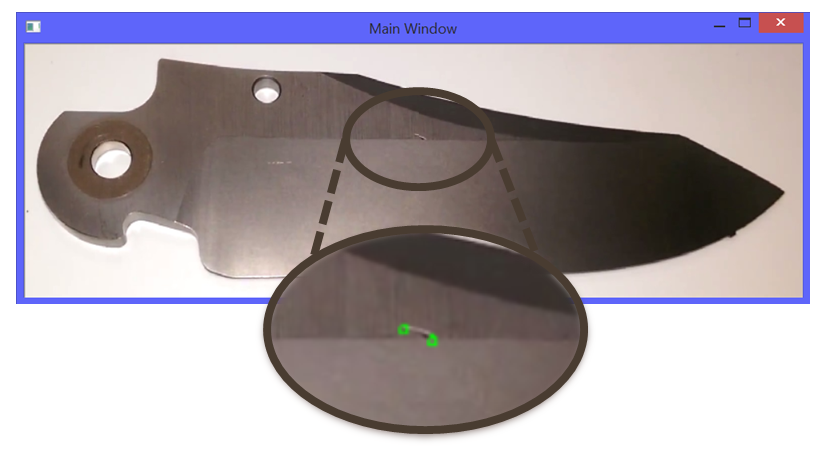
\includegraphics[width=.9\textwidth]{defect_location.png}
        \caption{Selected defect corners}
        \vspace*{2mm}
        \label{fig:defect corners}
    \end{subfigure}
    \hfill
    \begin{subfigure}[b]{.32\textwidth}
        \centering
        \raisebox{8.2mm}
        {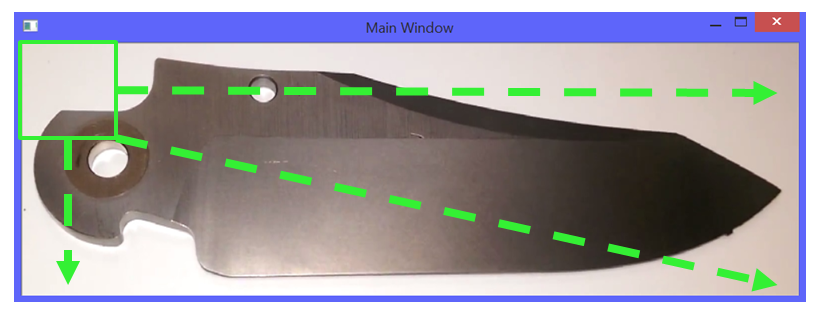
\includegraphics[width=.9\textwidth]{defect_sliding_window.png}}
        \caption{Sliding window}
        \vspace*{2mm}
        \label{fig:sliding window}
    \end{subfigure}
    \hfill
    \begin{subfigure}[b]{.32\textwidth}
        \centering
        \raisebox{1.7mm}
        {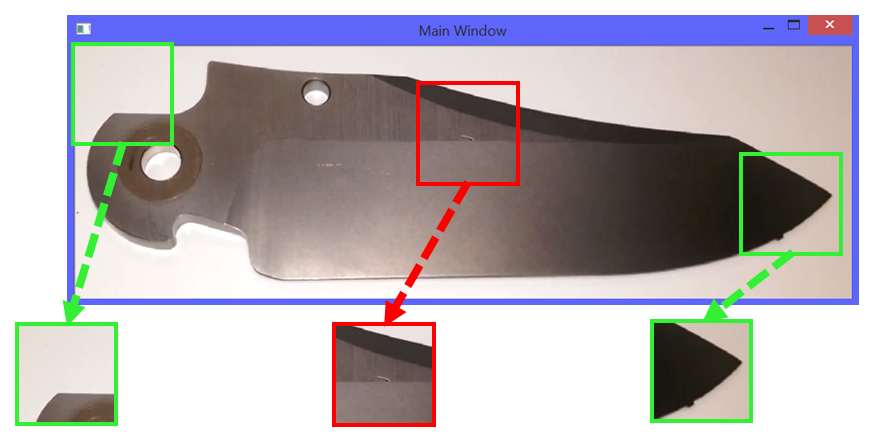
\includegraphics[width=.9\textwidth]{defect_windows.png}}
        \caption{Example labeled windows}
        \vspace*{2mm}
        \label{fig:labeled windows}
    \end{subfigure}
    \caption{Training data generation}
    \label{fig:data generation}
\end{figure*}

\subsection{Computer Vision Algorithm}

SUBSECTION TEXT

\begin{figure*}
    \centering
    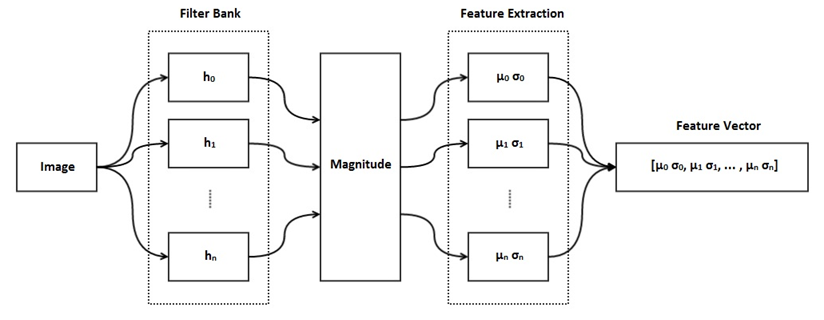
\includegraphics[width=.75\textwidth]{computer_vision_diagram.png}
    \caption{Computer vision algorithm flowchart}
    \vspace*{2mm}
    \label{fig:vision algorithm diagram}
\end{figure*}

\begin{figure}
    \centering
    \begin{subfigure}[b]{.49\textwidth}
        \centering
        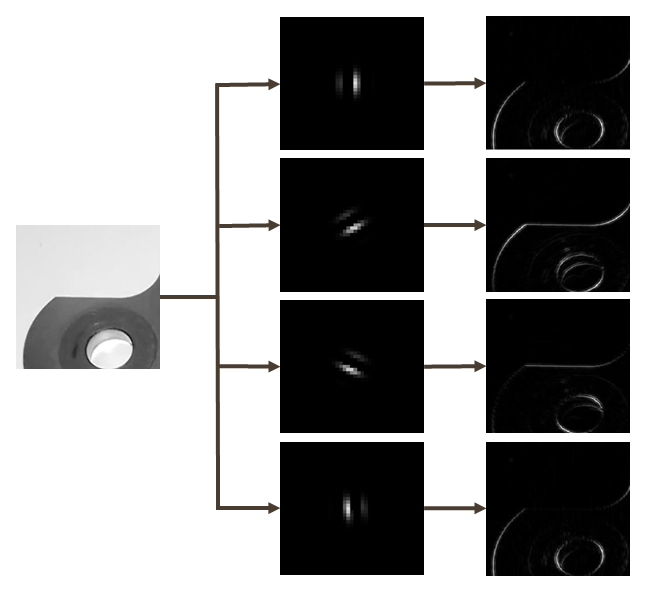
\includegraphics[width=.65\textwidth]{gabor_filter_small.png}
        \caption{Small Gabor filter bank}
        \vspace*{2mm}
        \label{fig:small gabor}
    \end{subfigure}
    \hfill
    \begin{subfigure}[b]{.49\textwidth}
        \centering
        {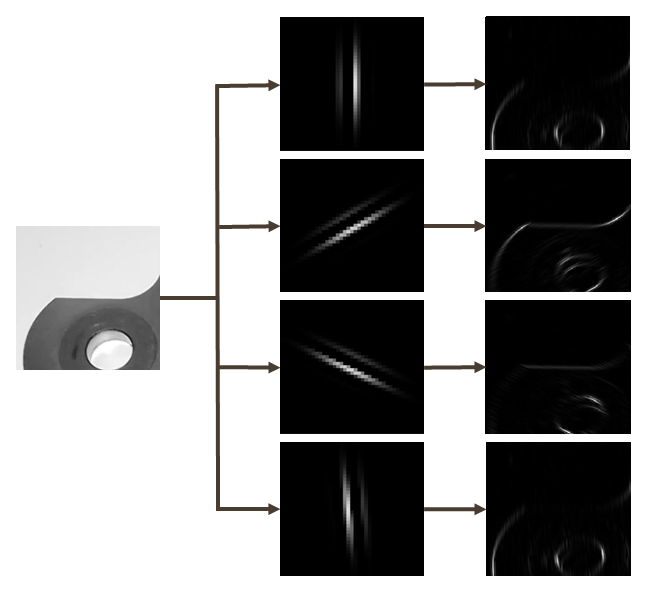
\includegraphics[width=.65\textwidth]{gabor_filter_large.png}}
        \caption{Large Gabor filter bank}
        \vspace*{2mm}
        \label{fig:large gabor}
    \end{subfigure}
    \caption{Gabor filter bank examples}
    \label{fig:gabor filter bank}
\end{figure}

\subsection{View Enumerations}

SUBSECTION TEXT

\subsection{Planning Algorithm}

SUBSECTION TEXT

\section{Results}

RESULTS TEXT

\subsection{SUBSECTION ONE}

SUBSECTION TEXT

\subsection{SUBSECTION TWO}

SUBSECTION TEXT

\section{Discussion}

\subsection{SUBSECTION ONE}

SUBSECTION TEXT

\section{Conclusion}

CONCLUSION TEXT

\bibliographystyle{IEEEtran}
\bibliography{main.bib}


\end{document}

% FIGURE HINTS 
%
%\begin{figure*}
%    \centering
%    \begin{subfigure}[b]{0.3\textwidth}
%        \centering
%        \includegraphics[width=.7\textwidth]{Reflex.jpg}
%        \caption{Reflex agent path}
%        \label{fig:reflex path}
%    \end{subfigure}
%    \hfill
%    \begin{subfigure}[b]{0.3\textwidth}
%        \centering
%        \includegraphics[width=.7\textwidth]{Random.jpg}
%        \caption{Random agent path}
%        \label{fig:random path}
%    \end{subfigure}
%    \hfill
%    \begin{subfigure}[b]{0.3\textwidth}
%        \centering
%        \includegraphics[width=.7\textwidth]{Memory.jpg}
%        \caption{Memory agent path}
%        \label{fig:memory path}
%    \end{subfigure}
%    \caption{Agent paths}
%    \label{fig:agent paths}
%\end{figure*}

% ALGORITHM HINTS
%
%\begin{algorithm}[h]
%\caption{Reflex agent}\label{reflex algorithm}
%\begin{algorithmic}[1]
%\If {$isDirty = true$}
%\State \Return \textit{actionSuck}
%\ElsIf {$facingWall \neq true$}
%\State \Return \textit{actionForward}
%\ElsIf {$facingWall = true$ AND $isHome = true$}
%\State \Return \textit{actionOff}
%\Else
%\State \Return \textit{actionTurnRight}
%\EndIf
%\end{algorithmic}
%\end{algorithm}